\section{DSLTrans}
\label{sec:DSLTrans_formal}

In this section we will introduce the DSLTrans transformation language and its
constructs from~\cite{DBLP:conf/sle/BarrocaLAFS10}. A formal treatment of the syntax and semantics of DSLTrans is found in \cref{sec:DSLTrans_formal_appendix}.

\subsection{DSLTrans Introduction}

DSLTrans is a visual graph-based and rule-based model
transformation engine that has two important properties enforced by construction: all its computations
are both \emph{terminating} and \emph{confluent}~\cite{Barroca2011}.
These properties stem from the fact that DSLTrans does not allow
unbounded loops during execution, making it a Turing-incomplete
computing language~\cite{Barroca2011}. Besides their obvious importance in
practice, \emph{termination} and \emph{confluence} were instrumental in the
implementation of our verification technique for pre-/post-condition contracts.

Model transformations are expressed in DSLTrans as sets of graph rewriting
rules, having an upper part (named \emph{MatchModel}), a lower part (\emph{ApplyModel}) and,
optionally, negative application conditions. The main construction
used in the scheduling of model transformation rules in DSLTrans is a
\emph{layer}. Each model transformation rule in a layer cannot match over the output of any other rule in the same layer. As well, rules cannot modify the input graph during the rewriting phase (termed \emph{out-place} execution). Layers are organized sequentially and
the output model that results from executing a given layer is passed as input to
the next layer in the sequence.

%Model transformations are expressed in DSLTrans as sets of graph rewriting
%rules, having the classical left-hand side (LHS), right-hand side (RHS) and,
%optionally, negative application conditions. The main construction
%used in the scheduling of model transformation rules in DSLTrans is a
%\emph{layer}: a layer contains a set of model transformation rules that execute
%without being able to see each other's output. This forces the rules in a layer
%to execute independently from each other. Layers are organized sequentially and
%the output model that results from executing a given layer is passed as input to
%the next layer in the sequence.

A DSLTrans rule can match over the elements of the input model of the
transformation and also over elements that have been generated so far in the
output model. Matching over elements of the output model of a
transformation is achieved using a DSLTrans construct called \emph{backward
links}. Backward links allow matching over traces between elements in the input and
the output models of the transformation. These traces are explicitly built by
the DSLTrans transformation engine during rule execution.

 \begin{figure}[t]
   \begin{center}
     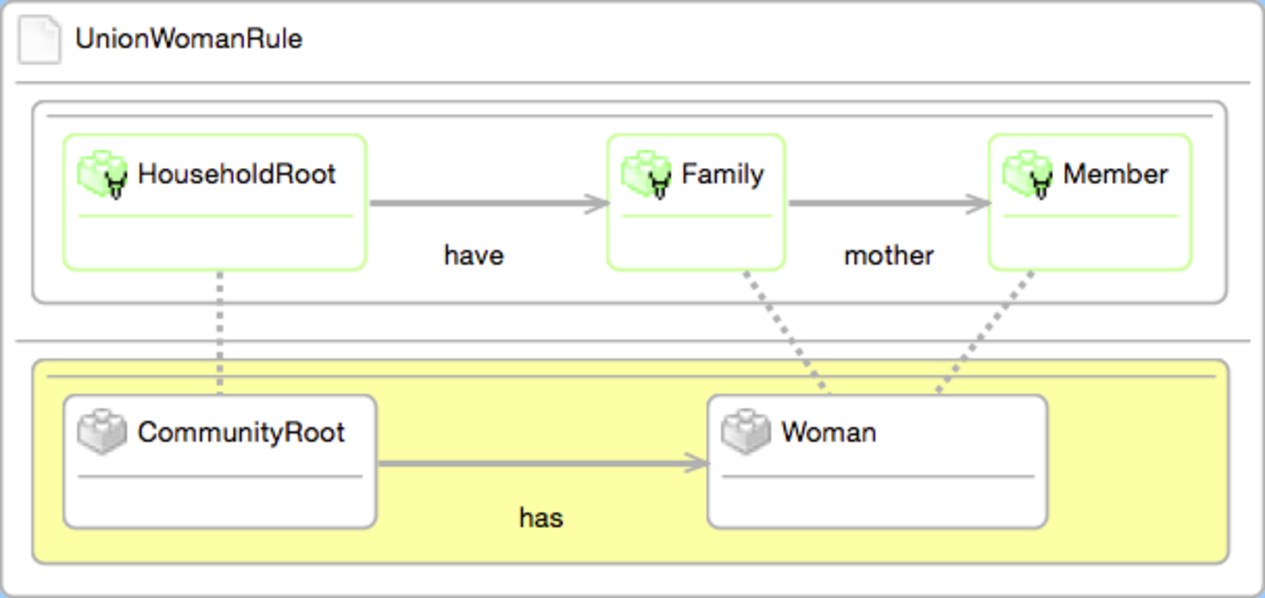
\includegraphics[width=0.40\textwidth]{figures/DSLTrans/UWRule.pdf}
     \caption{An example of a DSLTrans rule}
     \label{fig:DSLTrans_rule}
   \end{center}
   \vspace{-0.25in}
 \end{figure}

For example, we depict in Figure~\ref{fig:DSLTrans_rule} a
rule in the DSLTrans language.
When a rule is executed, the graph in the \emph{MatchModel} of the rule is searched for in the transformation's input model, together with the classes in the \emph{ApplyModel} of the rule that are connected to \emph{backward
links}. An example of a \emph{backward link} can be observed in
Figure~\ref{fig:DSLTrans_rule} as a dotted line connecting the \emph{Country} and the
\emph{Community} match classes. During the rewrite part of rule application,
the instances of classes in the \emph{ApplyModel} of the rule that are not connected to
backward links, together with their adjacent relations, are created in the
output model.

For example, the \emph{UnionWomanRule} rule in Figure~\ref{fig:DSLTrans_rule} will match over a \emph{Country} element connected to a \emph{Family} element connected to a \emph{Parent} element. If these elements are found in the input model along with the corresponding \emph{Community} and \emph{Woman} elements in the output model, then a \emph{persons} relation will be created between those output elements.

Although not present in this rule,
copying object attribute values from the \emph{MatchModel} to the \emph{ApplyModel} of the rules is
also part of the DSLTrans language, as illustrated in Section~\ref{sec:DSLTransRepresentation}.

\reviewer{Please explain, earlier on, the meaning of indirect edges.}


%\begin{figure*}[t]
%        \centering
%        \begin{subfigure}[b]{0.40\textwidth}
%                \centering
%                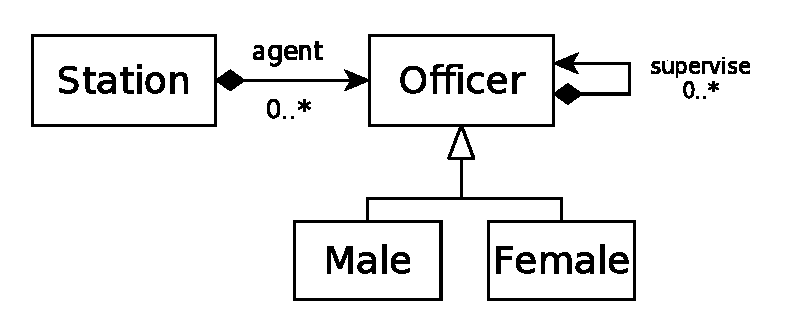
\includegraphics[width=1\textwidth]{./figures/policestation_dsltrans/organization.pdf}
%                \caption{Organization language}
%                \label{fig:OrganizationLanguage}
%        \end{subfigure}%
%        ~~
%        \begin{subfigure}[b]{0.40\textwidth}
%                \centering
%                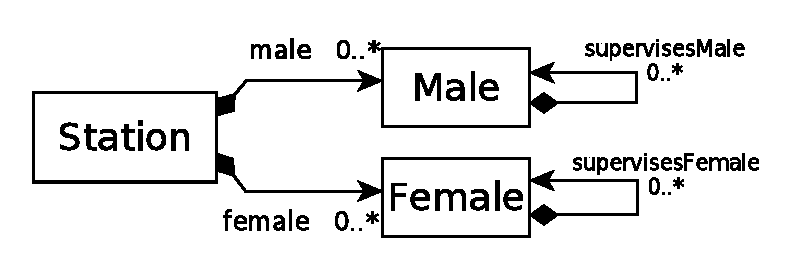
\includegraphics[width=1\textwidth]{./figures/policestation_dsltrans/gender.pdf}
%                \caption{Gender language}
%                \label{fig:GenderLanguage}
%        \end{subfigure}%
%        \caption{Metamodels for the Police Station transformation}
%        \label{fig:squadmetamodel}
%\end{figure*}

A DSLTrans transformation has a source and a target metamodel, which are seen
in \cref{fig:squadmetamodel}. This \emph{Police Station}
transformation will be presented throughout
the rest of this paper as an example transformation. The metamodel
in \cref{fig:OrganizationLanguage} represents a language for describing
the chain of command in a police station, which includes the male (\emph{Male}
class) and female officers (\emph{Female} class). The metamodel in
\cref{fig:GenderLanguage} represents a language for describing a different
view over the chain of command, where the officers working at the police station
are classified by gender.

\begin{figure*}[bht]
	\centering
		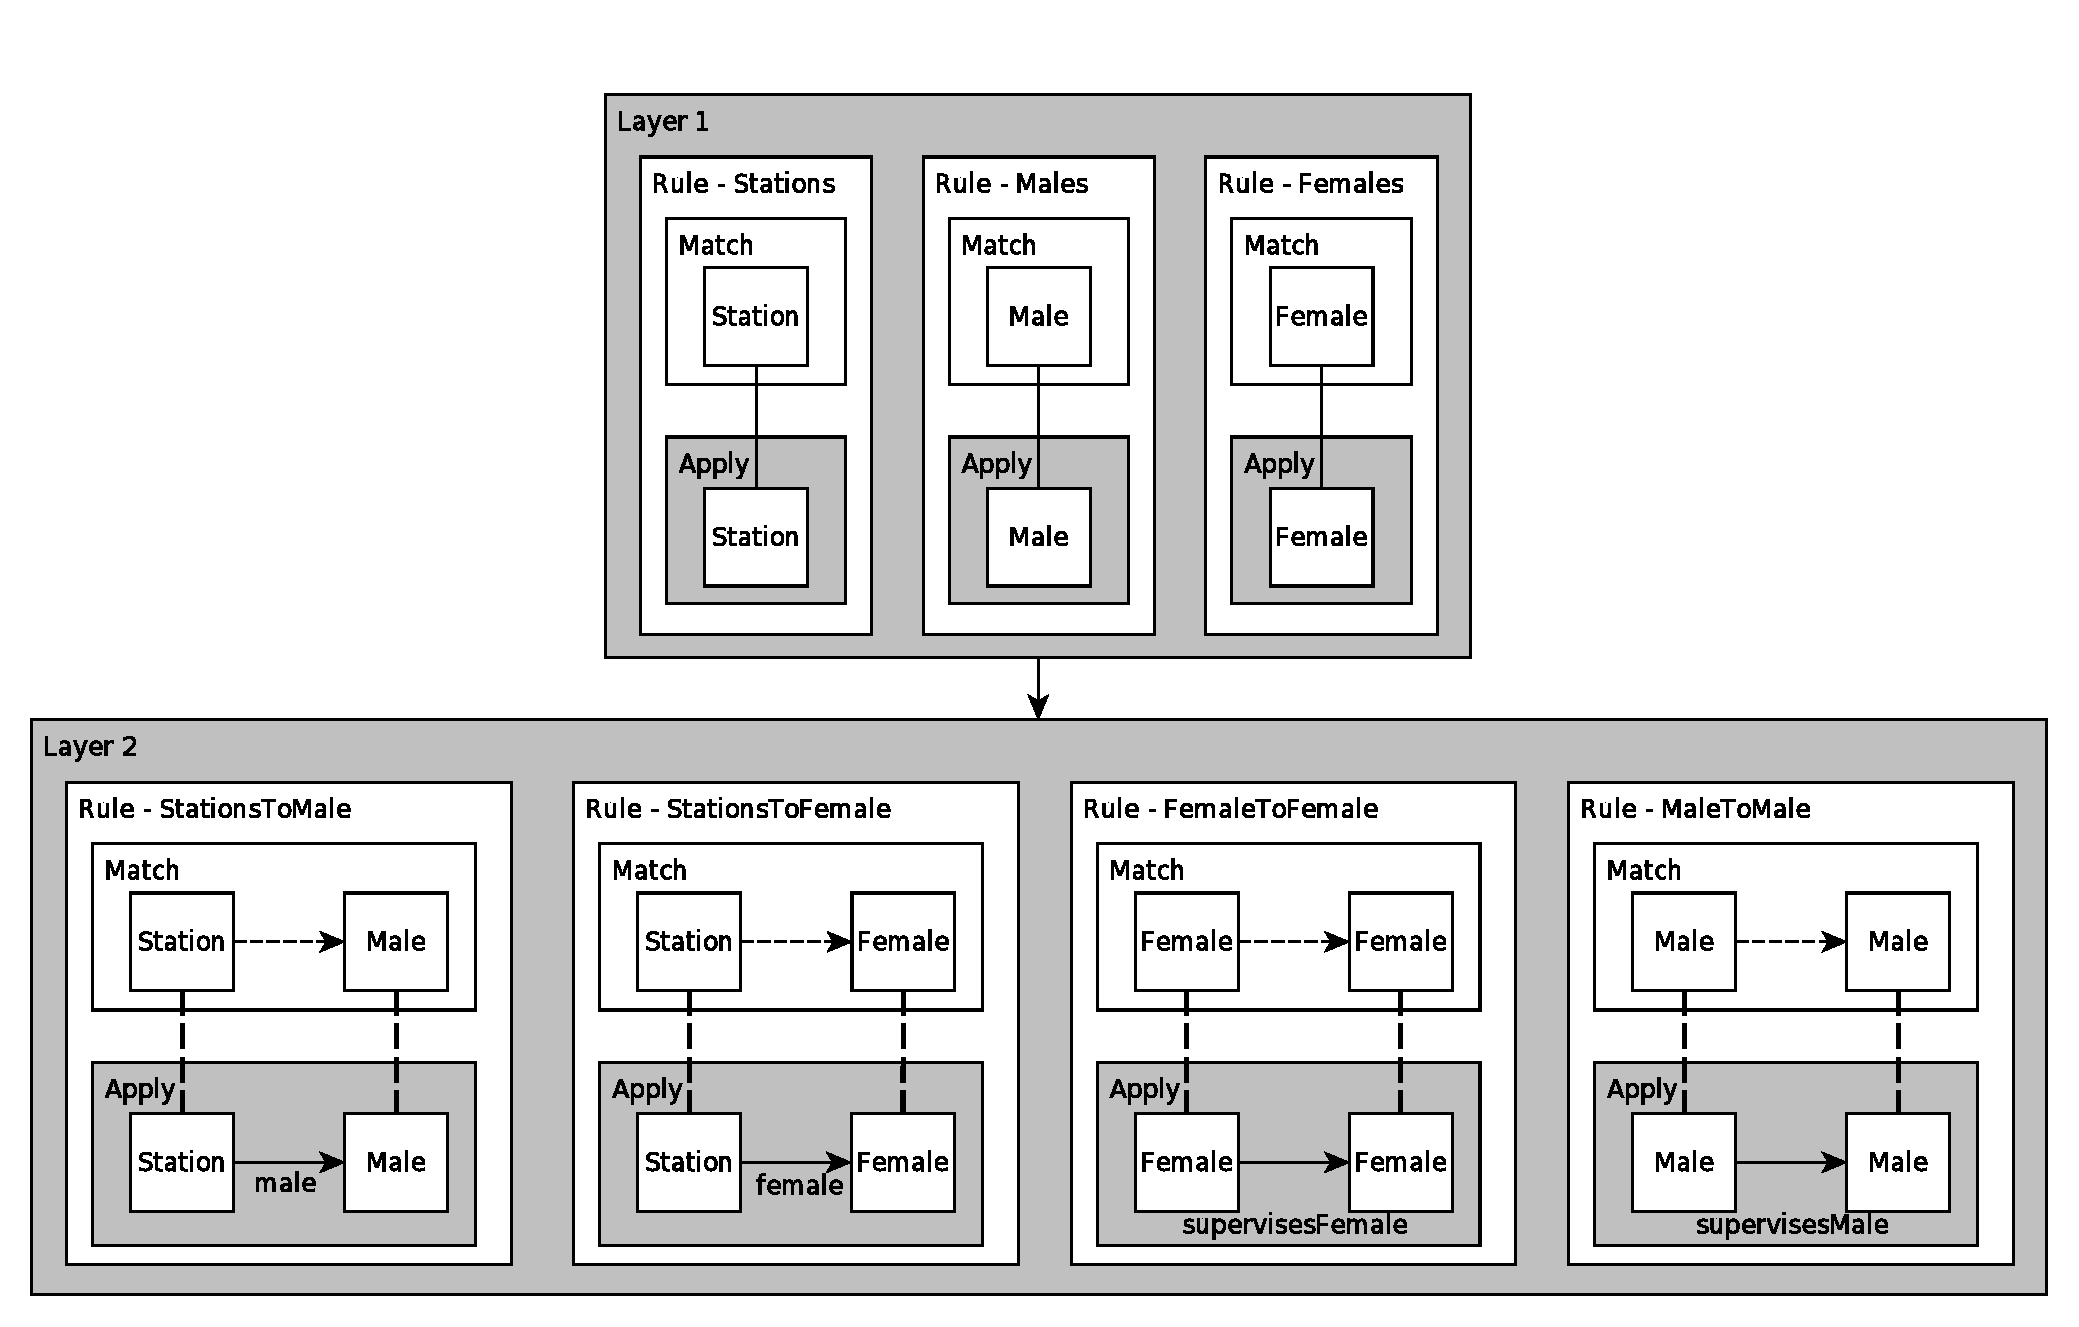
\includegraphics[width=0.9\textwidth]{./figures/policestation_dsltrans/transformation.pdf}
	\caption{The \emph{Police Station} model transformation expressed in DSLTrans}
	\label{fig:dsltransformation}
\end{figure*}

In \cref{fig:dsltransformation} we present a DSLTrans transformation that involves both metamodels.  A description of relevant constructs as well as visual notation remarks are found in \cref{subsec:DSLTrans_constructs}. Note
that the transformation is formed
from layers where each layer is a set of transformation rules. The
transformation will execute layer-by-layer, where transformation rules in a layer will execute in a
non-deterministic order but will always produce a deterministic result, due to the fact that DSLTrans is confluent by construction~\cite{DBLP:conf/sle/BarrocaLAFS10}.

Another important characteristic of DSLTrans transformations is that they are not Turing-complete. As discussed in~\cite{DBLP:conf/sle/BarrocaLAFS10}, non-completeness is required to make a transformation execution always terminate, but yet still allows for appropriate expressiveness.

Besides the fact that DSLTrans' transformations are free of constructs that
imply unbounded recursion or \\non-determinism, DSLTrans' transformations are strictly outplace, meaning no changes are allowed to the input model. However, the output metamodel for a DSLTrans transformation can
be the same as the input metamodel. Also, elements cannot be removed
from the output metamodel as the result of applying a DSLTrans rule.
This restriction is consistent with the usage of model transformations as
translations~\cite{AMT2012}, as no deletion of output elements is strictly required.

The purpose of this \emph{Police Station} transformation is to flatten a chain of command given
in the \emph{Organization language} into two independent sets of male
and female officers represented in the \emph{Gender language}. The command
relations will be kept during this transformation, i.e. a female officer will
have a direct association to all her female subordinates and likewise for male
officers. Note that differences in the gender classification metamodel mean
some relations present in the input model will not be retained in the output
model.

%\begin{figure*}[htb]
%        \centering
%        \begin{subfigure}[b]{0.30\textwidth}
%                \centering
%                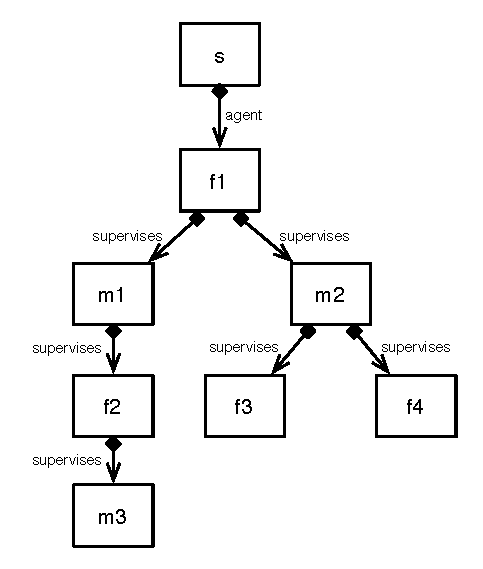
\includegraphics[width=1\textwidth]{./figures/policestation_dsltrans/model_police_hierarchy.pdf}
%                \caption{Original model}
%                \label{fig:police_hierarchy}
%        \end{subfigure}%
%        ~~
%        \begin{subfigure}[b]{0.40\textwidth}
%                \centering
%                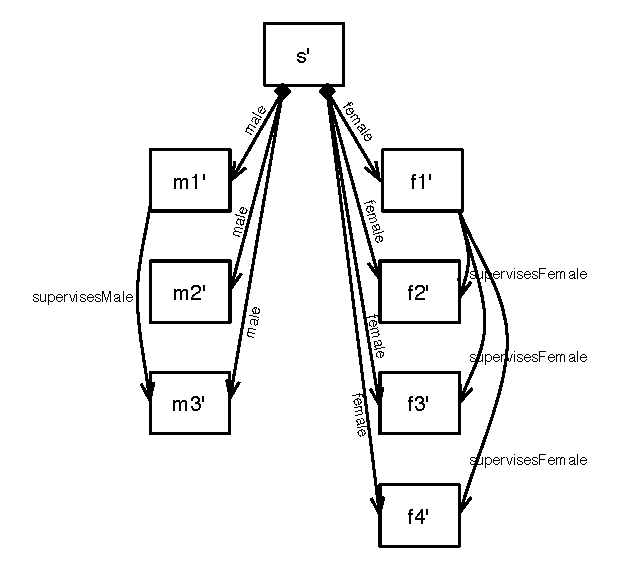
\includegraphics[width=1\textwidth]{./figures/policestation_dsltrans/model_police_gender.pdf}
%                \caption{Transformed model}
%                \label{fig:police_gender}
%        \end{subfigure}%
%        \caption{Model before and after transformation}
%        \label{fig:transformationexample}
%\end{figure*}
\reviewer{Figure 3: I would suggest adding another node f5 superviesd by f4, to illustrate the
notion of transitive closure. Another remark: I think the black containment dia-
monds do not belong in an instance model, as they are a metamodel notion.}

An example of this transformation's execution can be observed in \cref{fig:transformationexample}, where the input model is on the left and the output model is on the right. Notice that the elements $s$, $m_k$  and $f_k$ in \cref{fig:OrganizationLanguage} are instances of the source \emph{Organization} metamodel elements $Station$, $Male$ and $Female$ respectively. The primed elements in \cref{fig:police_gender} are their counterpart instances in the target \emph{Gender} metamodel.

Each individual transformation rule in the transformation is composed of two graphs. The first graph
is denoted as the \emph{match graph}, and is a pattern holding elements from the
source metamodel. Likewise, the \emph{apply graph} is a pattern containing
elements from the target metamodel. A formal definition of a transformation rule is found in~\cref{def:transformation_rule} in \cref{sec:formal_background}.

As an example, consider the transformation rule marked \emph{Stations} in the
first rule layer in \cref{fig:dsltransformation}. The match graph holds
one \emph{Station} element from the source metamodel, while the apply graph
holds one \emph{Station} element from the target metamodel. This means that for all
elements in the input model which are of type \emph{Station} in the
\emph{Organization Language}, an element of type
\emph{Station} in the \emph{Gender Language} will be created in the output model.

Note that in our approach, we require that the match graph of a rule is not a subgraph of the match graph of any other rule (as formally stated in \cref{def:layer_transformation} of model transformation, in \cref{sec:formal_background} of this paper). This requirement is to prevent the case where a rule could not execute independently of another rule, except for the cases when such dependency is explicitly defined by backward links. This is undesirable for the algorithm as presented here as we will explain later. However, as seen in~\cite{conf/gg/SelimLCDO14}, the expressiveness of the transformations our algorithm can examine \reviewer{Perhaps 'the expressiveness of the rule language'?}  is not restricted. In that work, we detail an operational rule processing step to handle overlapping rules.

\reviewer{In page 10 (answer to the reviewers) you say that rules for a 
  layer must be parallel independent. Is this written anywhere in the
  main part of the paper? }

In addition to the constructs presented in the example in
Figure~\ref{fig:DSLTrans_rule}, DSLTrans has several others:
\emph{existential matching} which allows selecting only one result when a match class of a rule
matches an input model, \emph{indirect links} for transitive matching
over containment relations in the input model, and \emph{negative application
conditions} that allow the transformation designer to specify conditions under
which a rule should not match. These constructs are not currently used in
our verification approach, and the interested reader is referred to~\cite{Barroca2011} for further information.

\subsection{DSLTrans Constructs}
\label{subsec:DSLTrans_constructs}
This section will describe all of the DSLTrans constructs involved in our
property-proving algorithm. These constructs are found in the transformation presented in \cref{fig:dsltransformation}. Formal details for the handled constructs are found in \cref{sec:DSLTrans_formal} and \cref{sec:DSLTrans_syntax}, while \cref{sec:DSLTrans_semantics} briefly introduces the formal semantics of this subset of DSLTrans. The visual syntax presented here is based on the DSLTrans Eclipse plug-in syntax~\cite{dsltrans_manual}.

\begin{itemize}
\item \textbf{Match Elements}: Match elements are variables typed by elements of the source
metamodel which will match over elements of that type (or subtype) in the
input model when the transformation is executed. Note that match
elements in a rule are searched for injectively in a model. This means that, for
example, if a match graph includes two elements of type \emph{Station}, then the rule will only match over models that include at least two instances of type \emph{Station}.

In the DSLTrans notation as seen throughout this paper, the match elements will be in a white box in the top half of a rule.\\

\item \textbf{Direct Match Links}: Direct match links are variables typed by labelled associations of the source metamodel, which will match over associations of the same type in the input model. A direct match link is always expressed between two match elements.\\

\item \textbf{Indirect Match Links}: Indirect match links are similar to direct
match links, but there may exist a path of containment associations between the
matched instances. Our notion of indirect links captures only
acyclic EMF containment associations. \reviewer{“a nonempty path” (I think). The label of the
containment associations does not matter?}

% As such, it avoids cycles and infinite
% amounts of matches over the transitive closure of associations in the input
% models.

In \cref{fig:dsltransformation}, indirect match links are represented in all the
transformation rules in the last layer as dashed arrows between elements in the match graph.\\

\item \textbf{Backward Links}: Backward links connect elements of the match and
the apply patterns of a DSLTrans rule in order to represent dependencies on
element creation by previous layers of the transformation. When used in a rule,
backward links match over traceability links between elements of the
transformation's input and output models.
These traceability links are implicitly created when any rule is executed during the transformation. Backward
links thus make it possible to refer in a rule to output elements created by a
previous layer.

Backward links are found in \cref{fig:dsltransformation} in all transformation rules on the last layer and are depicted as dashed lines.\\

%\item \emph{Negative Conditions}: it is possible to express negative conditions over
%match elements, backward, direct and indirect match links. 

\item \textbf{Apply Elements and Apply Links}: Apply elements and apply links are similar to match elements and
match links, but are instead typed by elements of the target metamodel. Apply elements in a given transformation rule that are not connected to backward links will create elements of the same type in the transformation's output. Apply links will always be created in the transformation's output. These output elements and links will be created as many times as the match graph of the rule is isomorphically found in the input model.\\

Consider the transformation rule denoted \emph{Station2Male} in the last rule
layer of \cref{fig:dsltransformation}. This rule takes \emph{Station} and
\emph{Male} elements of the \emph{Gender Language} metamodel, where these
elements were created in a previous layer from \emph{Station} and \emph{Male}
elements of the \emph{Organization Language} metamodel, and connects them using a
\emph{male} association.

%\item \emph{Apply Attributes}: DSLTrans includes a small language for
%building the values attributes of apply model elements from references to one or
%more match model element attributes.
\end{itemize}


\subsection{Families To Persons}

As our running example we present an extended version of the \FTP
transformation described in \cite{Oakes2015}. The original \FTP transformation can be
found in the ATL zoo~\cite{atlZoo}, and has also been discussed in a number of related works
on verification and testing~\cite{Gogolla2011}.

We chose this \FTP transformation as our running example for two reasons. First, it transforms domains whose concepts are easily understandable by anyone (cf. Section~\ref{sec:trans_domain}).
Second, it has a certain degree of complexity since it uses many features available in the ATL language (cf. Section~\ref{sec:trans_explanation}).

\subsection{Transformation Domains}\label{sec:trans_domain}

\begin{figure}[bt]
\centering
\subfigure[\emph{Families\_Extended} metamodel]{
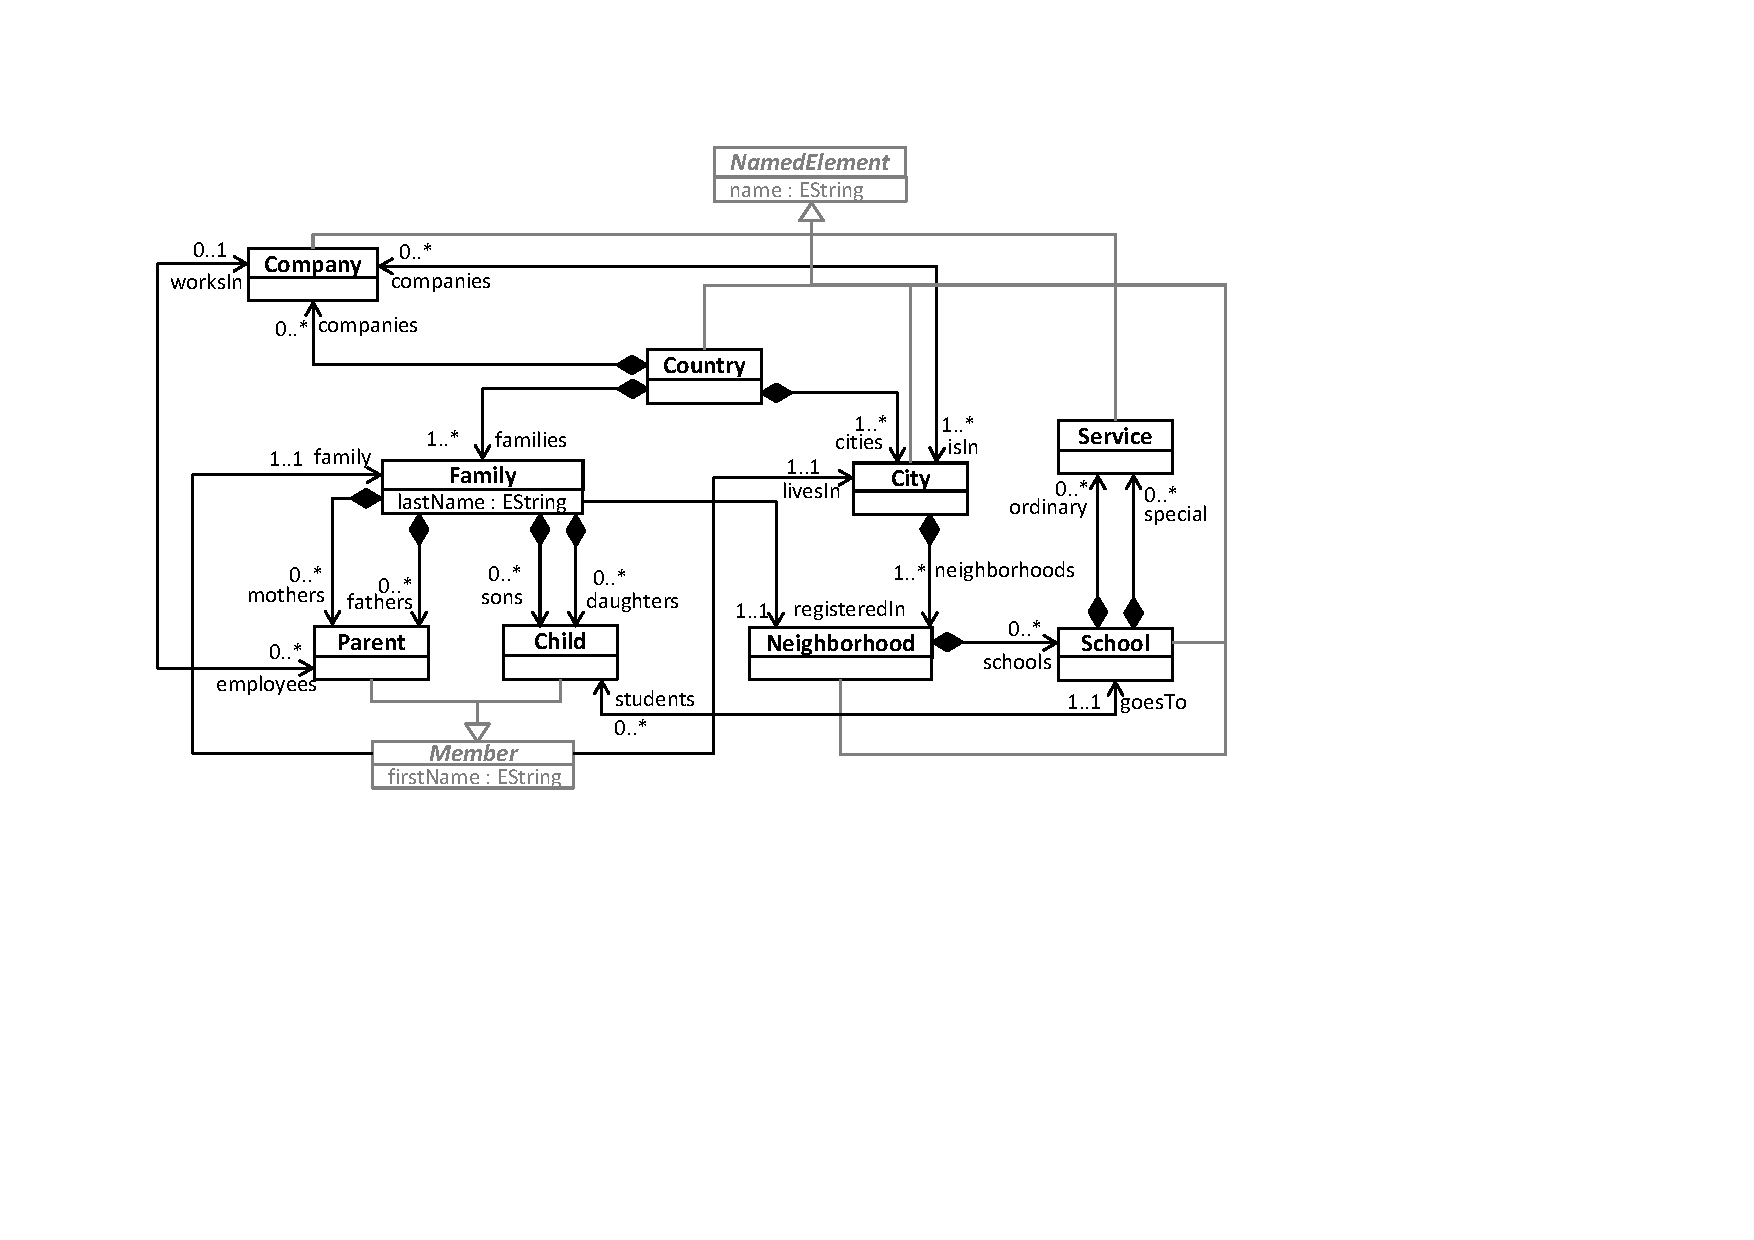
\includegraphics[width=0.97\columnwidth]{figures/DSLTrans/Families_Extended.pdf}
\label{fig:fams}
}
\subfigure[\emph{Persons\_Extended} metamodel]{
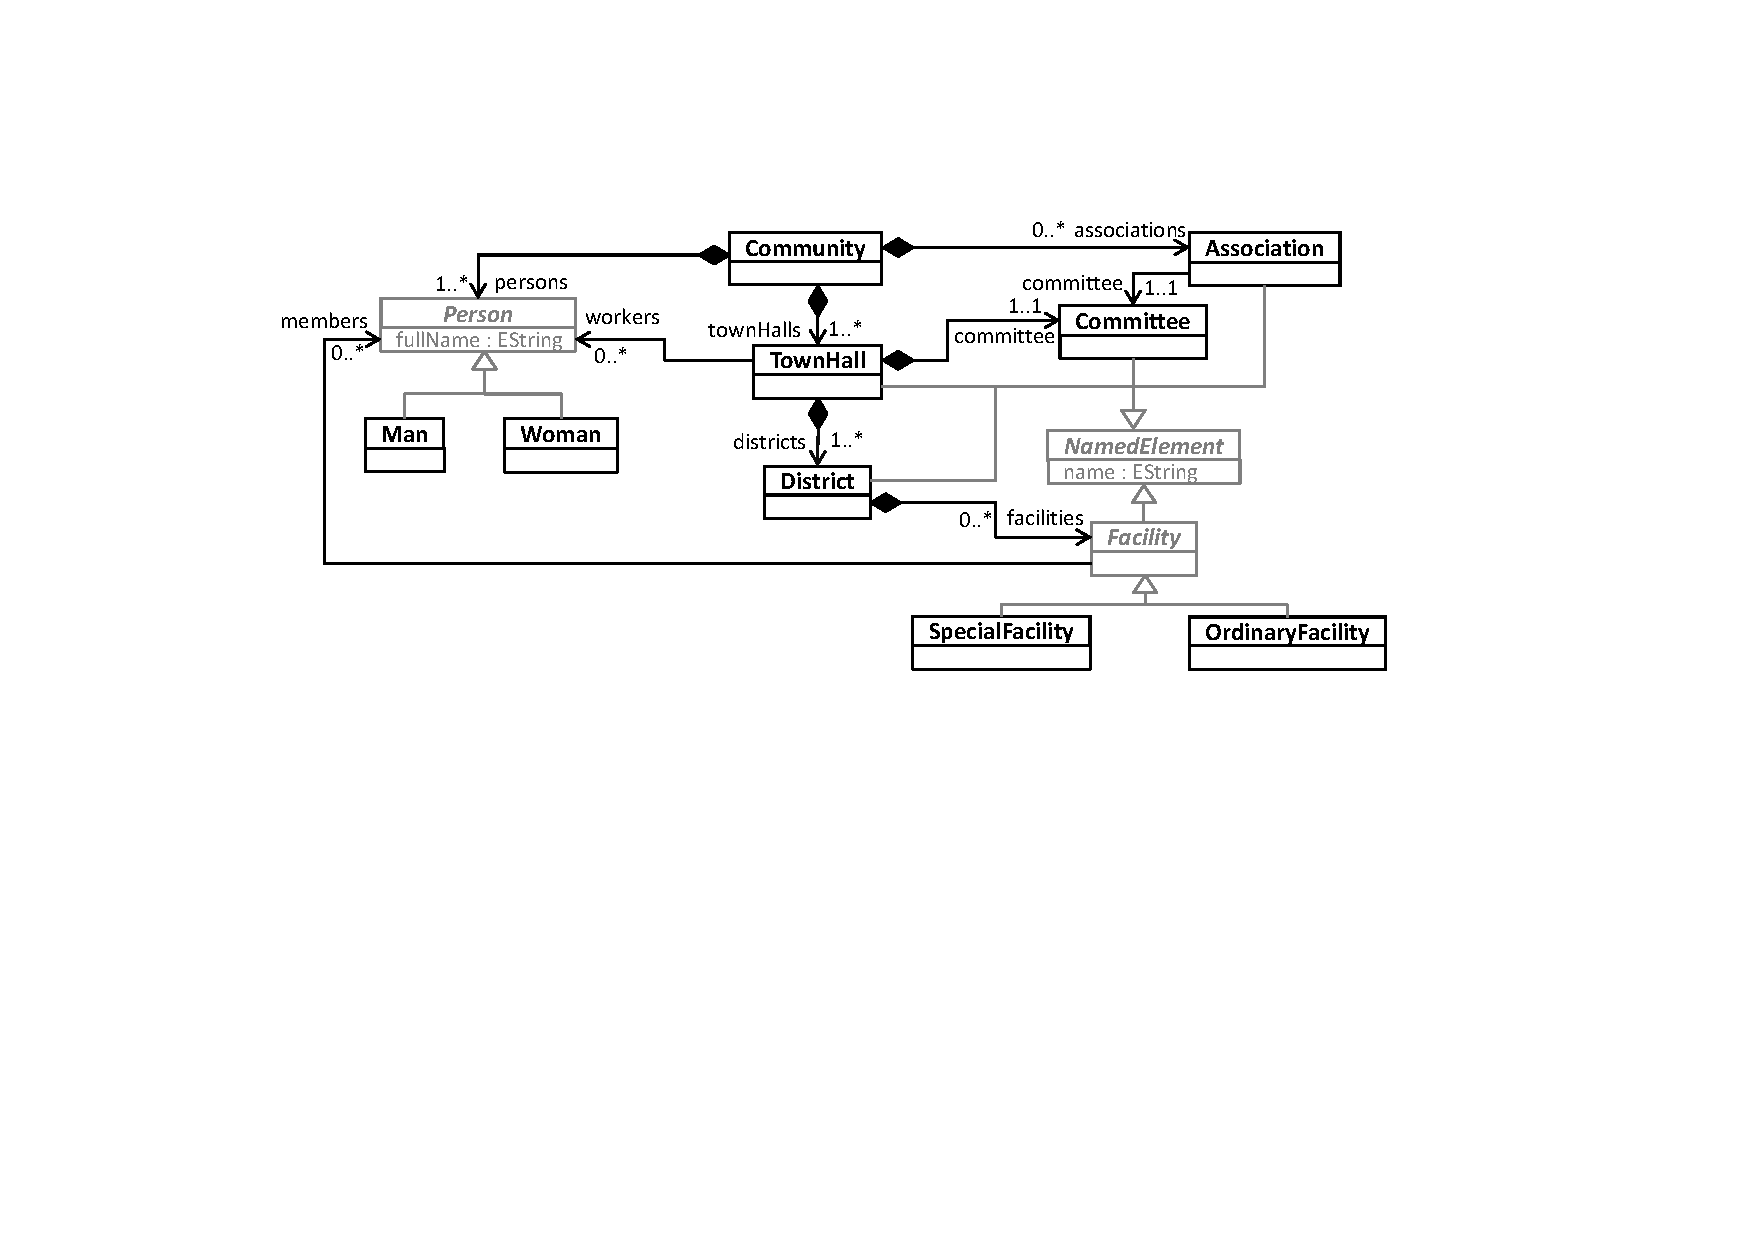
\includegraphics[width=0.97\columnwidth]{figures/DSLTrans/Persons_Extended.pdf}
\label{fig:pers}
}
\caption{Metamodels of the \emph{Families-to-Persons\_Extended} transformation}\label{fig:metamodels}
\end{figure}

The input and output metamodels of this transformation are shown in Figure~\ref{fig:metamodels}. Please note that abstract classes are depicted in grey color and with italic names, and inheritance relationships are depicted in grey.

The input metamodel, the \emph{Families\_Extended} metamodel, has the \emph{Country} class as a root element.
A \emph{Country} is made up of \emph{companies}, \emph{families} and \emph{cities}.
A \emph{Family} has a \emph{lastName}, is \emph{registeredIn} a \emph{Neighborhood} and can have any number of \emph{mothers} and \emph{fathers}, who are \emph{Parent}s and may, in turn, work in (\emph{worksIn}) a \emph{Company}.
It can also contain any number of \emph{sons} and \emph{daughters}, who are \emph{Child}ren, and every child \emph{goesTo} a \emph{School}.
Both parents and children are \emph{Member}s that have a \emph{firstName}, belong to a \emph{family} and each of them \emph{livesIn} a \emph{City}.

A \emph{City} may contain \emph{companies}, and a \emph{Company}, in turn, can be present in (relationship \emph{isIn}) several distinct cities.
A \emph{City} is composed of \emph{neighborhoods}, and these can have \emph{schools}, where several \emph{students} are registered.
Every \emph{School} has \emph{Service}s, and these may be \emph{special}, for students with special needs, or simply offer \emph{ordinary} services.
Finally, countries, cities, companies, neighborhoods and schools have a \emph{name} attribute, which is inherited from the abstract \emph{NamedElement} class.

The output metamodel, \emph{Persons\_Extended}, is shown in Figure~\ref{fig:pers}.
The root class is \emph{Community}, which is made up of \emph{persons}, \emph{townHalls} and \emph{associations}.
A \emph{Person} has a \emph{fullName} and can either be a \emph{Man} or a \emph{Woman}.
An \emph{Association} has a \emph{Committee} that makes decisions.
Every \emph{TownHall} has a roster of \emph{workers} (all the persons that are employed), hosts a \emph{Committee} to make decisions, and also governs several \emph{districts}.
A \emph{District} may contain several \emph{facilities}, either of type \emph{SpecialFacility} for those with special needs, or \emph{OrdinaryFacility}.
Each \emph{Facility} may have registered several persons as \emph{members}.
Finally, associations, town halls, committees, districts and facilities have a \emph{name} attribute.

\subsection{DSLTrans Representation}\label{sec:DSLTransRepresentation}

\begin{figure*}
  \begin{center}
  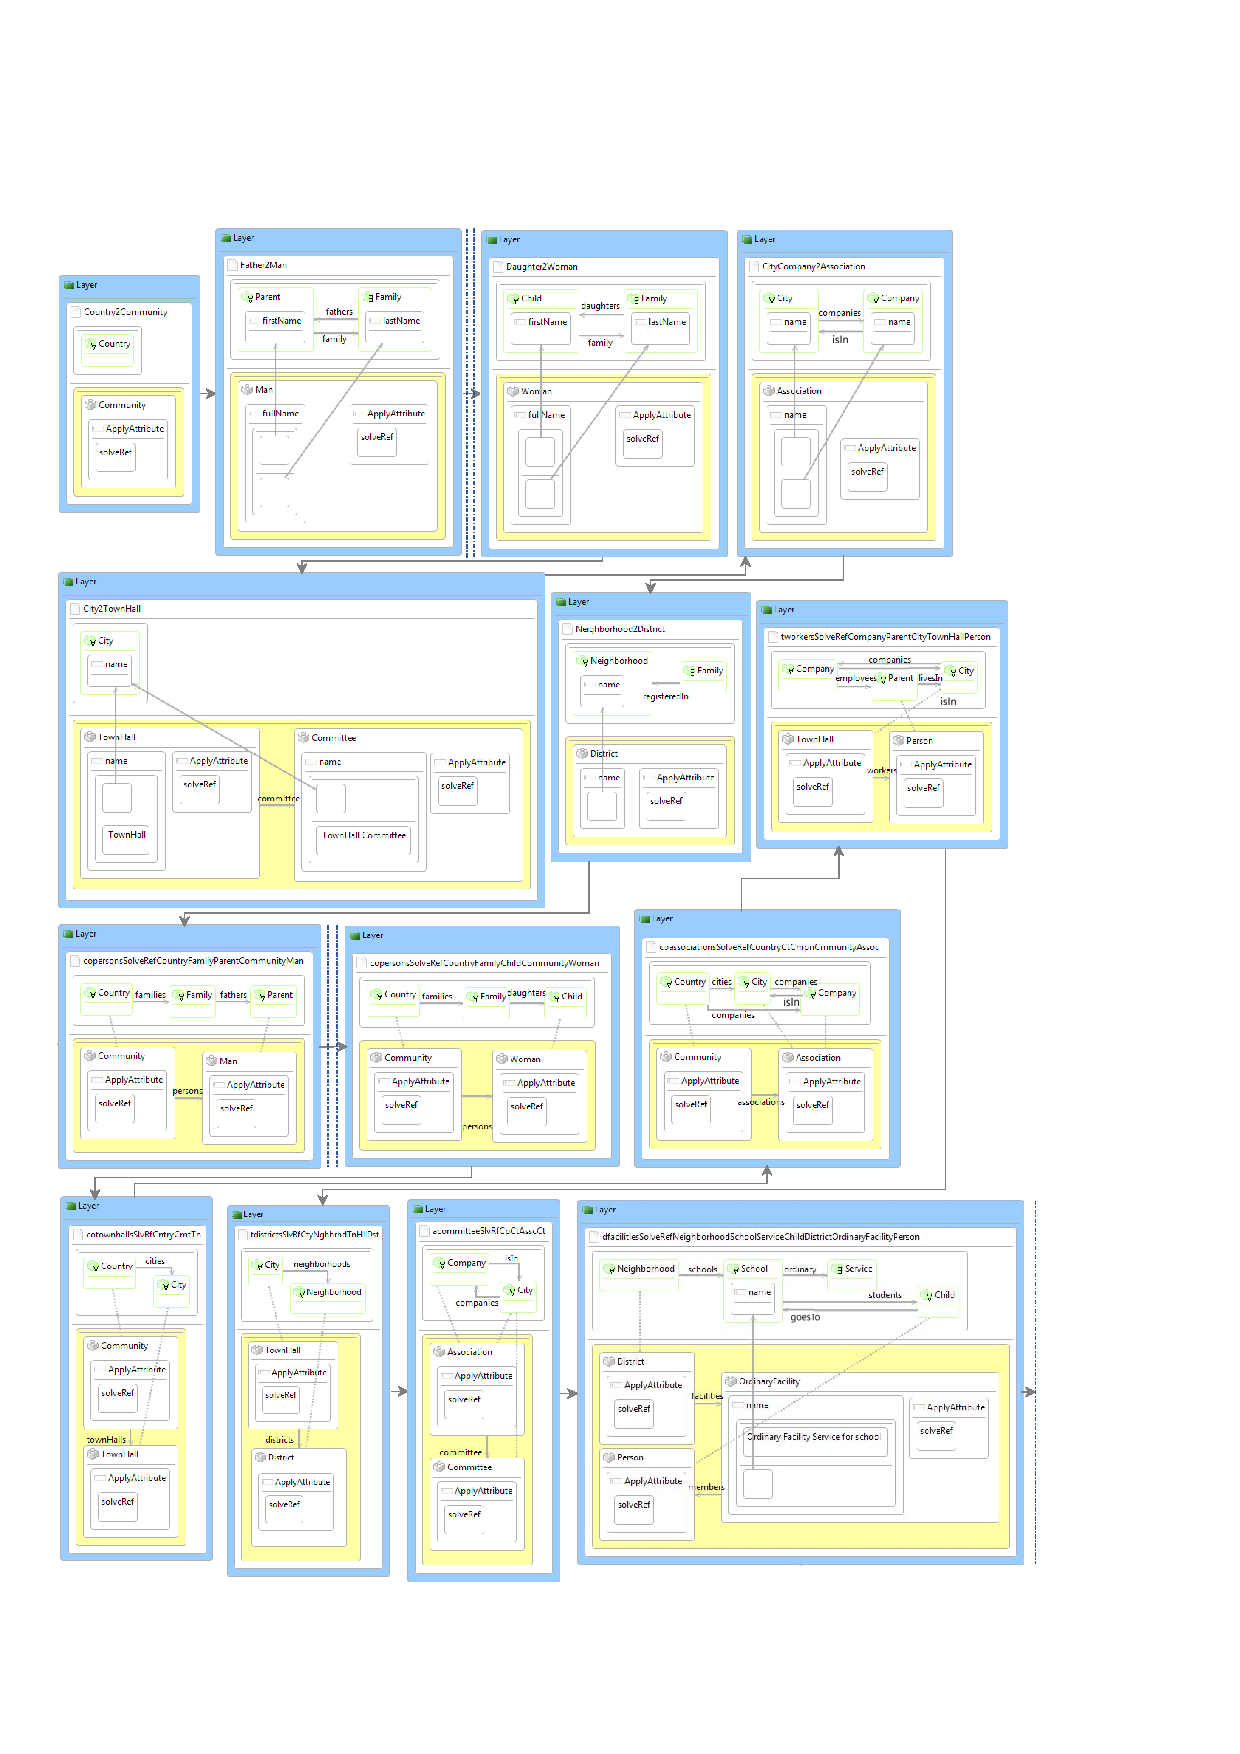
\includegraphics[width=0.94\textwidth]{figures/DSLTrans/DSLTrans_Rules_javi.pdf}
  \caption{DSLTrans version of the \emph{Families-to-Persons\_Extended} transformation}
  \label{fig:DSLTrans_rules}
  \end{center}
\end{figure*}


Figure~\ref{fig:DSLTrans_rules} displays the DSLTrans transformation which corresponds to the ATL \emph{Families-to-Persons\_Extended}\\
transformation shown in Listing~\ref{lst:F2P_Extended}. Let us mention here that we have removed five rules from the figure to improve visual clarity.
There is a vertical dotted blue line for each of these rules, located where the rules have been removed. The missed rules are similar to those that surround them, and can therefore be safely ignored in our explanation.

%As explained in Section~\ref{sec:dsltrans}, each DSLTrans rule has a \emph{MatchModel} and an \emph{ApplyModel}.
%As we can see, each of them has a left-hand side (LHS) and a right-hand side (RHS)\levi{not sure about the LHS/RHS reference here\ldots}.
%There are elements of a specific type and associations among them displayed in
% both the upper part (named \emph{MatchedModel} in DSLTrans) and lower part (called \emph{ApplyModel}) of the rules.
%In each side, elements of a specific type and relationships among them are displayed.
%Elements can also have attributes.
%Rule \emph{Households2Community} corresponds to rule R1 in
%Listing~\ref{lst:Families2Persons}, \emph{Father2Man} corresponds to rule R2 and \emph{UnionFather}
%to binding B11.

%They appear in the \emph{ApplyModel} when they have to be initialized, and
%in the \emph{MatchedModel} when they are used to initialize attributes in the \emph{ApplyModel}.
%For instance, attributes \emph{fullName} and \emph{lastName} of \emph{Member} and \emph{Family} in rule \emph{Father2Man} are used
%to initialize attribute \emph{fullName} of \emph{Man}.
%%
%%Other than these attributes, there are others in the RHS which appear in an element
%%whenever such element is going to be used in backward links, and they also appear when they are being used in such links. These attributes are always referred to with the name \emph{ApplyAttribute}.
%%For instance, we can see in rule \emph{Households2Community}, which is created for R1 in Listing~\ref{lst:Families2Persons}, that a \emph{Community} is created for a \emph{Households}.
%%Besides, since these two elements are going to be used later in a backward link, the \emph{ApplyAttribute} attribute is set in \emph{Community}. Note that the \emph{ApplyAttribute} attribute of an element must be created when the element is created, and the rule where it is created must be in the sequence of rules before the rule that uses the element in a backward link.
%
%Rule \emph{Households2Community} corresponds to R1 in
%Listing~\ref{lst:Families2Persons}, although the reference \emph{has} is not
%initialized in this rule.
%
%Rule \emph{Father2Man} corresponds to R2. We can see how the two elements in the
%\emph{from} part of the ATL rule appear in the \emph{MatchedModel} of the DSLTrans rule, as well
%as the filter used in ATL, which is represented as an association. The
%element \emph{Man} appears in the \emph{ApplyModel}, and its \emph{fullName} attribute is
%updated with the concatenation of the \emph{firstName} and \emph{lastName}
%attributes. A similar rule, not shown here, creates elements of type
%\emph{Woman}, which corresponds to R3 in Listing~\ref{lst:Families2Persons}.
%
%The last rule is used to set the \emph{has} relation between a \emph{Community}
%and a \emph{Man}. Here, backward links are used. The first one is to indicate
%that the \emph{Community} element has been created from a \emph{Households}
%element (which was done in rule \emph{Households2Community}). The other two
%backward links state that the \emph{Man} is created from a \emph{Family} and a
%\emph{Member} that are linked with the relation \emph{father} (such as in rule
%\emph{Father2Man}). This rule corresponds to binding B11 in
%Listing~\ref{lst:Families2Persons}. There is a similar rule, not shown in the
%figure, for initializing the \emph{has} association between \emph{Community} and
%\emph{Woman}, what corresponds to B12.

The process of constructing a DSLTrans transformation from an ATL one is described in the next section.
For now, note that DSLTrans transformation obtained from ATL through the higher-order transformation includes only one rule per layer, meaning all rules execute sequentially.
This is due to the sequential semantics of ATL that we replicate in DSLTrans.


Also, note that attribute copies are represented with arrows from the \emph{ApplyModel} of the rule to the \emph{MatchModel}, such as in rule \emph{Neighborhood2District}, where the created \emph{District} gets the same name as the matched \emph{Neighborhood}.
The string of an attribute of a created element can also be initialized with the concatenation of several strings.
For instance, in rule \emph{Father2Man}, the full name of the created \emph{Man} comes from the concatenation of the first name of the matched \emph{Parent} and the last name of his/her \emph{Family}.
Or it can be assigned the string of an attribute of an element in the \emph{MatchModel} concatenated with a given string, such as in rule \emph{City2TownHall}.



%\emph{Father2Man} in Figure~\ref{fig:DSLTrans_transformation} performs an attribute
%copy from the match to the apply part of the rule, graphically represented with arrows from the \emph{ApplyModel} to the \emph{MatchModel}. More precisely, it
%fills in the \emph{fullName} attribute of the generated \emph{Man} instance by
%concatenating the \emph{firstName} and \emph{lastName} attribute values found
%respectively in the \emph{member} and \emph{family} instances identified by the
%match part of the rule. This operation replicates the concatenation of the
%\emph{firstName} and the \emph{lastName} occurring in the rule component marked
%\emph{B2} in Listing~\ref{lst:Families2Persons}.

%The first three rules in the DSLTrans transformation replicate the R1, R2, and R3
% portions of the ATL transformation. Then, the last four rules in
% Figure~\ref{fig:DSLTrans_transformation} connect those elements and set the values, replicating B11, B12, B2, and B3 in Listing~\ref{lst:Families2Persons}.
%
% This transformation has been built automatically from its ATL
%counterpart using a higher-order transformation, which will be presented in Section~\ref{sec:mapping}. For now, we will briefly the differences and
%similarities between the two transformations:
%
%\begin{itemize}
%  \item The DSLTrans F2P transformation is completely graphical, while the ATL
%  F2P transformation is fully textual.
%  \item The DSLTrans F2P is composed of layers that are organized sequentially.
%  A layer in DSLTrans is a box (e.g. the \emph{Root} rule in
%  Figure~\ref{fig:DSLTrans_transformation}) that can contain one or more rules.
%  In the transformation in Figure~\ref{fig:DSLTrans_transformation}) each layer
%  contains only one rule, as that layout is automatically produced by the higher
%  order transformation.
%  \item The layers belonging to the transformation in
%  Figure~\ref{fig:DSLTrans_transformation} execute one after the other, passing
%  the result of one layer to the next one.
%\end{itemize}


\subsection{Formal Structures}



This section will detail the abstract syntax of the constructs involved in a DSLTrans transformation.

As discussed in Section~\ref{subsec:DSLTrans_syntax}, DSLTrans transformations are composed of rules arranged in layers.

\subsubsection{Similar Structures}

Note that in the definitions that follow, in this section and others, that we define structures which are very similar in composition, which each containing two or three typed graphs, as well as a link component. This similarity is essential to our technique, as we will define morphisms between the various components of these constructions, which vary depending on the particular structure under examination.

While this composition of typed graph approach is preferred by the authors due to its reflection in our prover implementation, some readers may disagree. In this case, note that it is equivalent to think of these structures as one large typed graph annotated by the component it originates from, with appropriate projections for selecting relevant portions.


\subsubsection*{DSLTrans Transformation Rule}

A transformation rule is the elemental block of a DSLTrans transformation. Several transformation rules can be observed in the Police Station transformation in \cref{fig:dsltransformation}.

A transformation rule includes a non-empty match pattern and a non-empty apply pattern. This is also known in the model transformation literature as a rule's \emph{left hand side} and \emph{right hand side}. As described in Section 3.4 or Section 2, which the match graph elements are found in the input model, then the apply graph elements are produced in the output model.

A match pattern can include indirect links that are used to transitively match containment relations in a model. The apply pattern of a rule always contains at least one apply element that is not connected to a backward link or an edge, meaning in practice that a rule will always produce something and not only match. An apply pattern does not include indirect links as it is used only for the construction of parts of instances of a metamodel.

A rule may also contain a negative application condition (NAC) which if matched over the target graph prevents application of the rule.

A transformation rule also includes backward links, as informally introduced in \cref{subsec:DSLTrans_constructs}. As described in that section, backward links define dependencies between rules. \bentley{Expand}


\begin{definition}{DSLTrans Transformation Rule\\}
\label{def:transformation_rule}

A DSLTrans transformation rule is a four-tuple $\big\langle \mathit{NAC}$, $\mathit{Match}$, $\mathit{Apply}$, $\mathit{backward}\big\rangle$, where:

\begin{itemize}
\item $\mathit{NAC}$, $\mathit{Match}, \mathit{Apply} \in \textsc{TG}$
\item $\mathit{Match}$ and $\mathit{Apply} $ are non-empty and are disjoint
\item $\mathit{NAC}$ may be an empty graph, and is disjoint from both $\mathit{Match}$ and $\mathit{Apply} $

\end{itemize}  

Note that when we require an element of the $\mathit{Match}$, $\mathit{Apply}$, or $\mathit{NAC}$ graphs, such as the vertices, we will index the required element. For example, the vertices for the \textit{Match} graph will be $V_{\textit{Match}}$.

\begin{itemize}
\item $\mathit{backward} = \{E_{back}, (s_{back}, t_{back})\}$
\item $E_{back}$ contains the backward links
\begin{itemize}
\item $E_{back} $ is disjoint from $E_{Match}$,  $E_{Apply}$, and $E_{NAC}$
\end{itemize}
\item $(s_{back}, t_{back})$ is a pair of functions $s_{back}: E_{back}\rightarrow V_{\textit{Apply}}$ and $t_{back}: E_{back}\rightarrow V_{\textit{Match}}$ that respectively provide the pattern and target vertices for each backward link
\begin{itemize}
\item Note the source of backward links is a vertex in $V_{\textit{Apply}}$ while the target is a vertex in $V_{\textit{Match}}$
\end{itemize}
\end{itemize}

\textsc{Rules} is the set of all rules.

\end{definition}

We additionally impose that for the well-formedness of a DSLTrans rule, there always exists an element or edge to be created in the \textit{Apply} graph to be created. That is, either there are edges to be created in the \textit{Apply} graph, or there is a vertex in the \textit{Apply} graph that is not the source of a backward link.

\begin{itemize}
\item $E_{\textit{Apply}} \neq \emptyset \lor$
\item $ \exists v \in V_{\textit{Apply}} | \big\{\forall e \in E_{back}: s_{back}(e) \neq v \big\}$
\end{itemize}



\subsubsection*{DSLTrans Layer and Transformation}

\cref{def:layer} and \cref{def:transformation} formalise the abstract syntax of a model transformation, introduced in \cref{sec:dsltrans}. An example of a model transformation can be observed in \cref{fig:dsltransformation}, the Police Station transformation. As expected, a DSLTrans transformation is composed of a sequence of layers where each layer is composed of a set of rules.

\begin{definition}{Layer\\}
\label{def:layer}
A layer is a finite set of transformation rules: $\{r_0, r_1, \dots, r_n | r_i \in \textsc{Rules}\}$.

The set of all layers is denoted $\textsc{Layers}$. 
\end{definition}

Note that the order of the rules within the layer does not matter, due to the semantics of DSLTrans rule execution. As discussed in Section BLAH, these semantics ensure that rules are independent, and cannot act on the output of other rules within the same layer.

\begin{definition}{DSLTrans Transformation\\}
\label{def:transformation}

A DSLTrans transformation is a finite list of layers denoted $\{l_0, l_1, \dots, l_n | l \in \textsc{Layers}\}$. Note that the order of layers in a transformation is important.

The set of all transformations is denoted $\textsc{Transforms}$.



\end{definition}



\subsubsection*{Input-Output Model}

To describe the semantics of a DSLTrans model transformation, we must define an \textit{input-output model} construct. This input-output model allows the representation of the initial state as well as intermediate operational states during the execution of a model transformation. These input-output models are thus the `path conditions' which represent all transformation executions through an abstraction relation. This is further discussed in Section ABSTRACTION RELATION.

The structure of a input-output model is intentionally very similar to a DSLTrans rule. There is one typed graph representing the input model and another typed graph representing the output model. As well, the construct contains a set of edges, named \emph{traceability links}, for keeping a history of which elements in the output model originated from which elements in the input model.

\begin{definition}{Input-Output Model\\}
\label{def:input_output_model}

An input-output model rule is a three-tuple $\big\langle \mathit{Input}$, $\mathit{Output}$, $\mathit{trace}\big\rangle$, where:

\begin{itemize}
\item $\mathit{Input}, \mathit{Output} \in \textsc{TG}$
\item $\mathit{Input}$ and $\mathit{Output} $ may be empty and are disjoint
\item $\mathit{trace} = \{E_{trace}, (s_{trace}, t_{trace})\}$
\begin{itemize}
\item $E_{trace}$ contains the traceability links
\item $E_{trace} $ is disjoint from $E_{Input}$ and $E_{Output}$
\item $(s_{trace}, t_{trace})$ is a pair of functions $s_{trace}: E_{trace}\rightarrow V_{\textit{Output}}$ and $t_{trace}: E_{trace}\rightarrow V_{\textit{Input}}$ that respectively provide the source and target vertices for each traceability link
\end{itemize}

\end{itemize}  

Let $\mathit{IOM}$ be the set of all input-output models.

We define a utility function getTransformation: IOM $\rightarrow$ Transforms. This function returns the Transform that the input-output model was built for. The purpose of this function is to restrict input-output models to only be applicable for the transformation they represent.

Note that the $\VT$ and $\ET$ for input and output will come from the input and output metamodels. \bentley{Expand} 

\end{definition}


\subsection{Transformation Semantics}
\label{sec:DSLTrans_semantics}

This section will discuss the semantics of a DSLTrans transformation. Given an input model and a transformation, an output layer will be produced through the repeated execution of rules and layers.



\subsubsection*{Execution of a DSLTrans Rule}

We will now address the execution of a rule in the DSLTrans language, basing our explanation on double pushouts.

Note that we will apply rules differently, depending on whether they contain indirect links or not. We will begin with the simpler case where the rule does not contain indirect links, diagrammed in Figure~\ref{fig:dpo}.

We create first the matcher and the rewriter for a DSLTrans rule.


\subsubsection*{Matcher of a Transformation Rule}

To create the actual matcher construct that will be matched during a rule's execution, the rule's \textit{Match} graph is combined with backward links, as well as any \textit{Apply} vertices connected to the backward links.

Note that the rule's NAC will also be considered in the matching of a rule.

\begin{definition}{Matcher of a Transformation Rule\\}
\label{def:matcher_transformation_rule}

Let the transformation rule $r = \big\langle \mathit{NAC}$, $\mathit{Match}$, $\mathit{Apply}$, $\mathit{backward}\big\rangle$.

We define $r$'s matcher, noted $\lceil r \rceil$, to be a typed graph six-tuple $\langle V,E,(s,t),\tau, \VT, \ET\rangle$, where:
\begin{itemize}
\item $V = V_{Match} \cup \big\{v \in V_{Apply} | \{\exists e \in E_{back} | s_{back}(e) = v\}\big\}$
\item $E = E_{Match} \cup E_{back}$
\item $s = s_{Match} \cup s_{back}$, $t = t_{Match} \cup t_{back}$
\item $\tau = \tau_{Match} \cup \tau_{Apply}$
\item $\VT = \VT_{Match} \cup \VT_{Apply}$
\item $\ET = \ET_{Match} \cup \ET_{Apply}$
\end{itemize}

\end{definition}

\subsubsection*{Rewriter of a Transformation Rule}

To continue with the double pushout approach, we must construct the rewriting (or replacement) graph.

The construction of this rewriter is essentially the same as the underlying rule. However, to support traceability, we require that backward links in the rule be converted into traceability links, and that new traceability links be created between all match and apply vertices. 

\begin{definition}{Rewriter of a Transformation Rule\\}
\label{def:rewriter_transformation_rule}

Let the transformation rule $r = \big\langle \mathit{NAC}$, $\mathit{Match}$, $\mathit{Apply}$, $\mathit{backward}\big\rangle$.

We define $r$'s rewriter, noted $\lfloor r \rfloor$, to be a structure $\big\langle \mathit{Input}$, $\mathit{Output}$, $\mathit{trace}\big\rangle$, where:

\begin{itemize}
\item $ \mathit{Input} = \mathit{Match}$
\item $ \mathit{Output} = \mathit{Apply}$
\end{itemize}

We then modify $\mathit{trace}$ to contain the appropriate traceability links

\begin{itemize}
\item $E_{trace} = \exists e \in E_{trace} | $
\begin{itemize}
\item $ \forall m \in V_{Match}, a \in V_{Apply}:$$s_{trace}(e) = a$, $t_{trace}(e) = m$ 
\end{itemize}
\end{itemize}

\end{definition}

\subsubsection*{Double-Pushout Approach}

\begin{figure}[h!] \centering
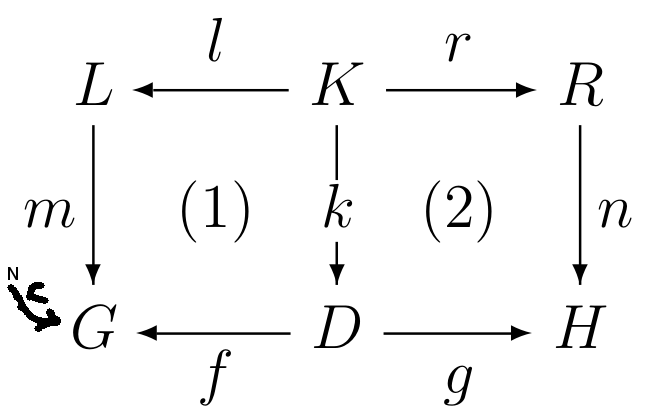
\includegraphics[width=0.44\textwidth]{figures/formal/dpo_with_NAC}
	\caption{Double pushout approach}
	\label{fig:dpo}
\end{figure}


If the reader is unfamiliar with the theory of double-pushouts, we refer to work on Fundamentals of Algebraic Graph Transformation.

The core idea of double-pushouts is to present graph rewriting in terms of morphisms, which compartmentalize the actions of finding a match and adding/deleting edges.

The application of a rule is called a \textit{production}. Below, we will first explain the production of a single DSLTrans rule, expand this production to handle indirect links in the rule, then discuss multiple productions.

Let this production be for a rule $r = \langle \mathit{NAC}, \mathit{[Match}, \mathit{Apply}, \mathit{back} \rangle$. To simplify the explanation, we constrain our rules to not include any indirect links. That is, $\nexists E \in E_{\textit{Match}} \cup E_{\mathit{NAC}} | \mathit{isIndirect}(E)$.

Figure~\ref{fig:dpo} presents a basic diagram for the approach.
The major components are:
\begin{itemize}
\item L: The matcher of the rule $\lceil r \rceil$
\item R: The rewriter of the rule $\lfloor r \rfloor$
\item G: The graph to be matched/rewritten
\item H: The rewritten graph
\end{itemize}

\paragraph{Rule Components}
K is the interface graph between L and R. That is, elements in K appear in both L and R. Elements which are to be deleted by the production appear in L but not K, and elements to be created are present in R but not K.

In the absence of indirect links, we note that $K = L$ as elements cannot be deleted in DSLTrans rules. Therefore the morphism l is isomorphism.

The morphism r from K to R is an injective typed graph homomorphism. Note that as described in Section~\ref{subsubsec:structure_homomorphism}, this homomorphism will be composed of sub-homomorphisms between the $\mathit{Match} \rightarrow \mathit{Input}$, $\mathit{Apply} \rightarrow \mathit{Output}$, and $\mathit{backward} \rightarrow \mathit{trace}$.

N represents the typed graph NAC of the rule. We note that this production cannot occur if there is a typed graph edge homomorphism c between the rule's NAC and G. 


\paragraph{Graph Components}

G is the target graph which is to be matched on.

m is the typed graph homomorphism between the matcher of a rule $r$, denoted ($\lceil r \rceil$) and the $\mathit{Input}$ component of the input-output model.

D is the interface graph between the original graph G, and the rewritten graph H. Similar to K, D contains elements in both. Again, as DSLTrans rules do not delete elements, D will be isomorphic to G in this case, and f will be isomorphism. The morphism k will embed the K interface graph within the interface graph D.

The morphism g from the interface graph D to the rewritten graph H gives the graph elements, while the morphism $r$ gives the embedding of the rewriter R with the elements to be produced. Thus, it is the pushout of R and D through K that gives H. g and n will be typed graph morphisms.


\subsubsection{Double-Pushout Approach with Indirect Links}

If the DSLTrans rule contains indirect links, we must modify the double-pushout approach described above to handle the transitive closure that the construct implies. The main change is to build the transitive edges, match on them, and then not build them in the final graph.

Note that this second explanation is valid for rules containing indirect links, or not containing them. 

\begin{figure}[h!] \centering
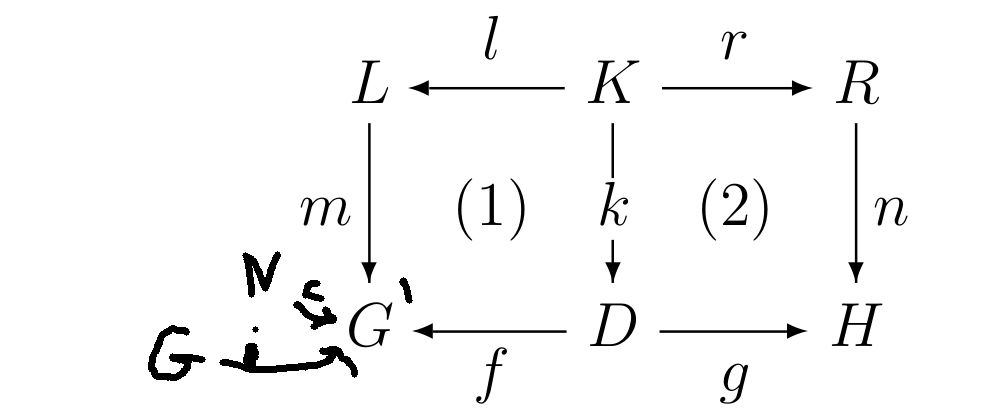
\includegraphics[width=0.44\textwidth]{figures/formal/dpo_with_NAC_and_indirect}
	\caption{Double pushout approach with indirect links}
	\label{fig:dpo_indirect}
\end{figure}

We add the component G' to the diagram, which represents the transitive closure of the Input graph of G. The homomorphism i gives the embedding of G into G'.

The homomorphism m will try to map the indirect links onto the newly created edges in G'.

K will not contain the indirect links. Therefore l will not longer be surjective, as nothing will map to the indirect links. R and r remain the same.

The interface D does not contain the edges newly created in G'. Thus the morphism f does not map onto these edges in G'.

n, g, and H remain the same.

\paragraph{Example}


\begin{figure}[h!] \centering
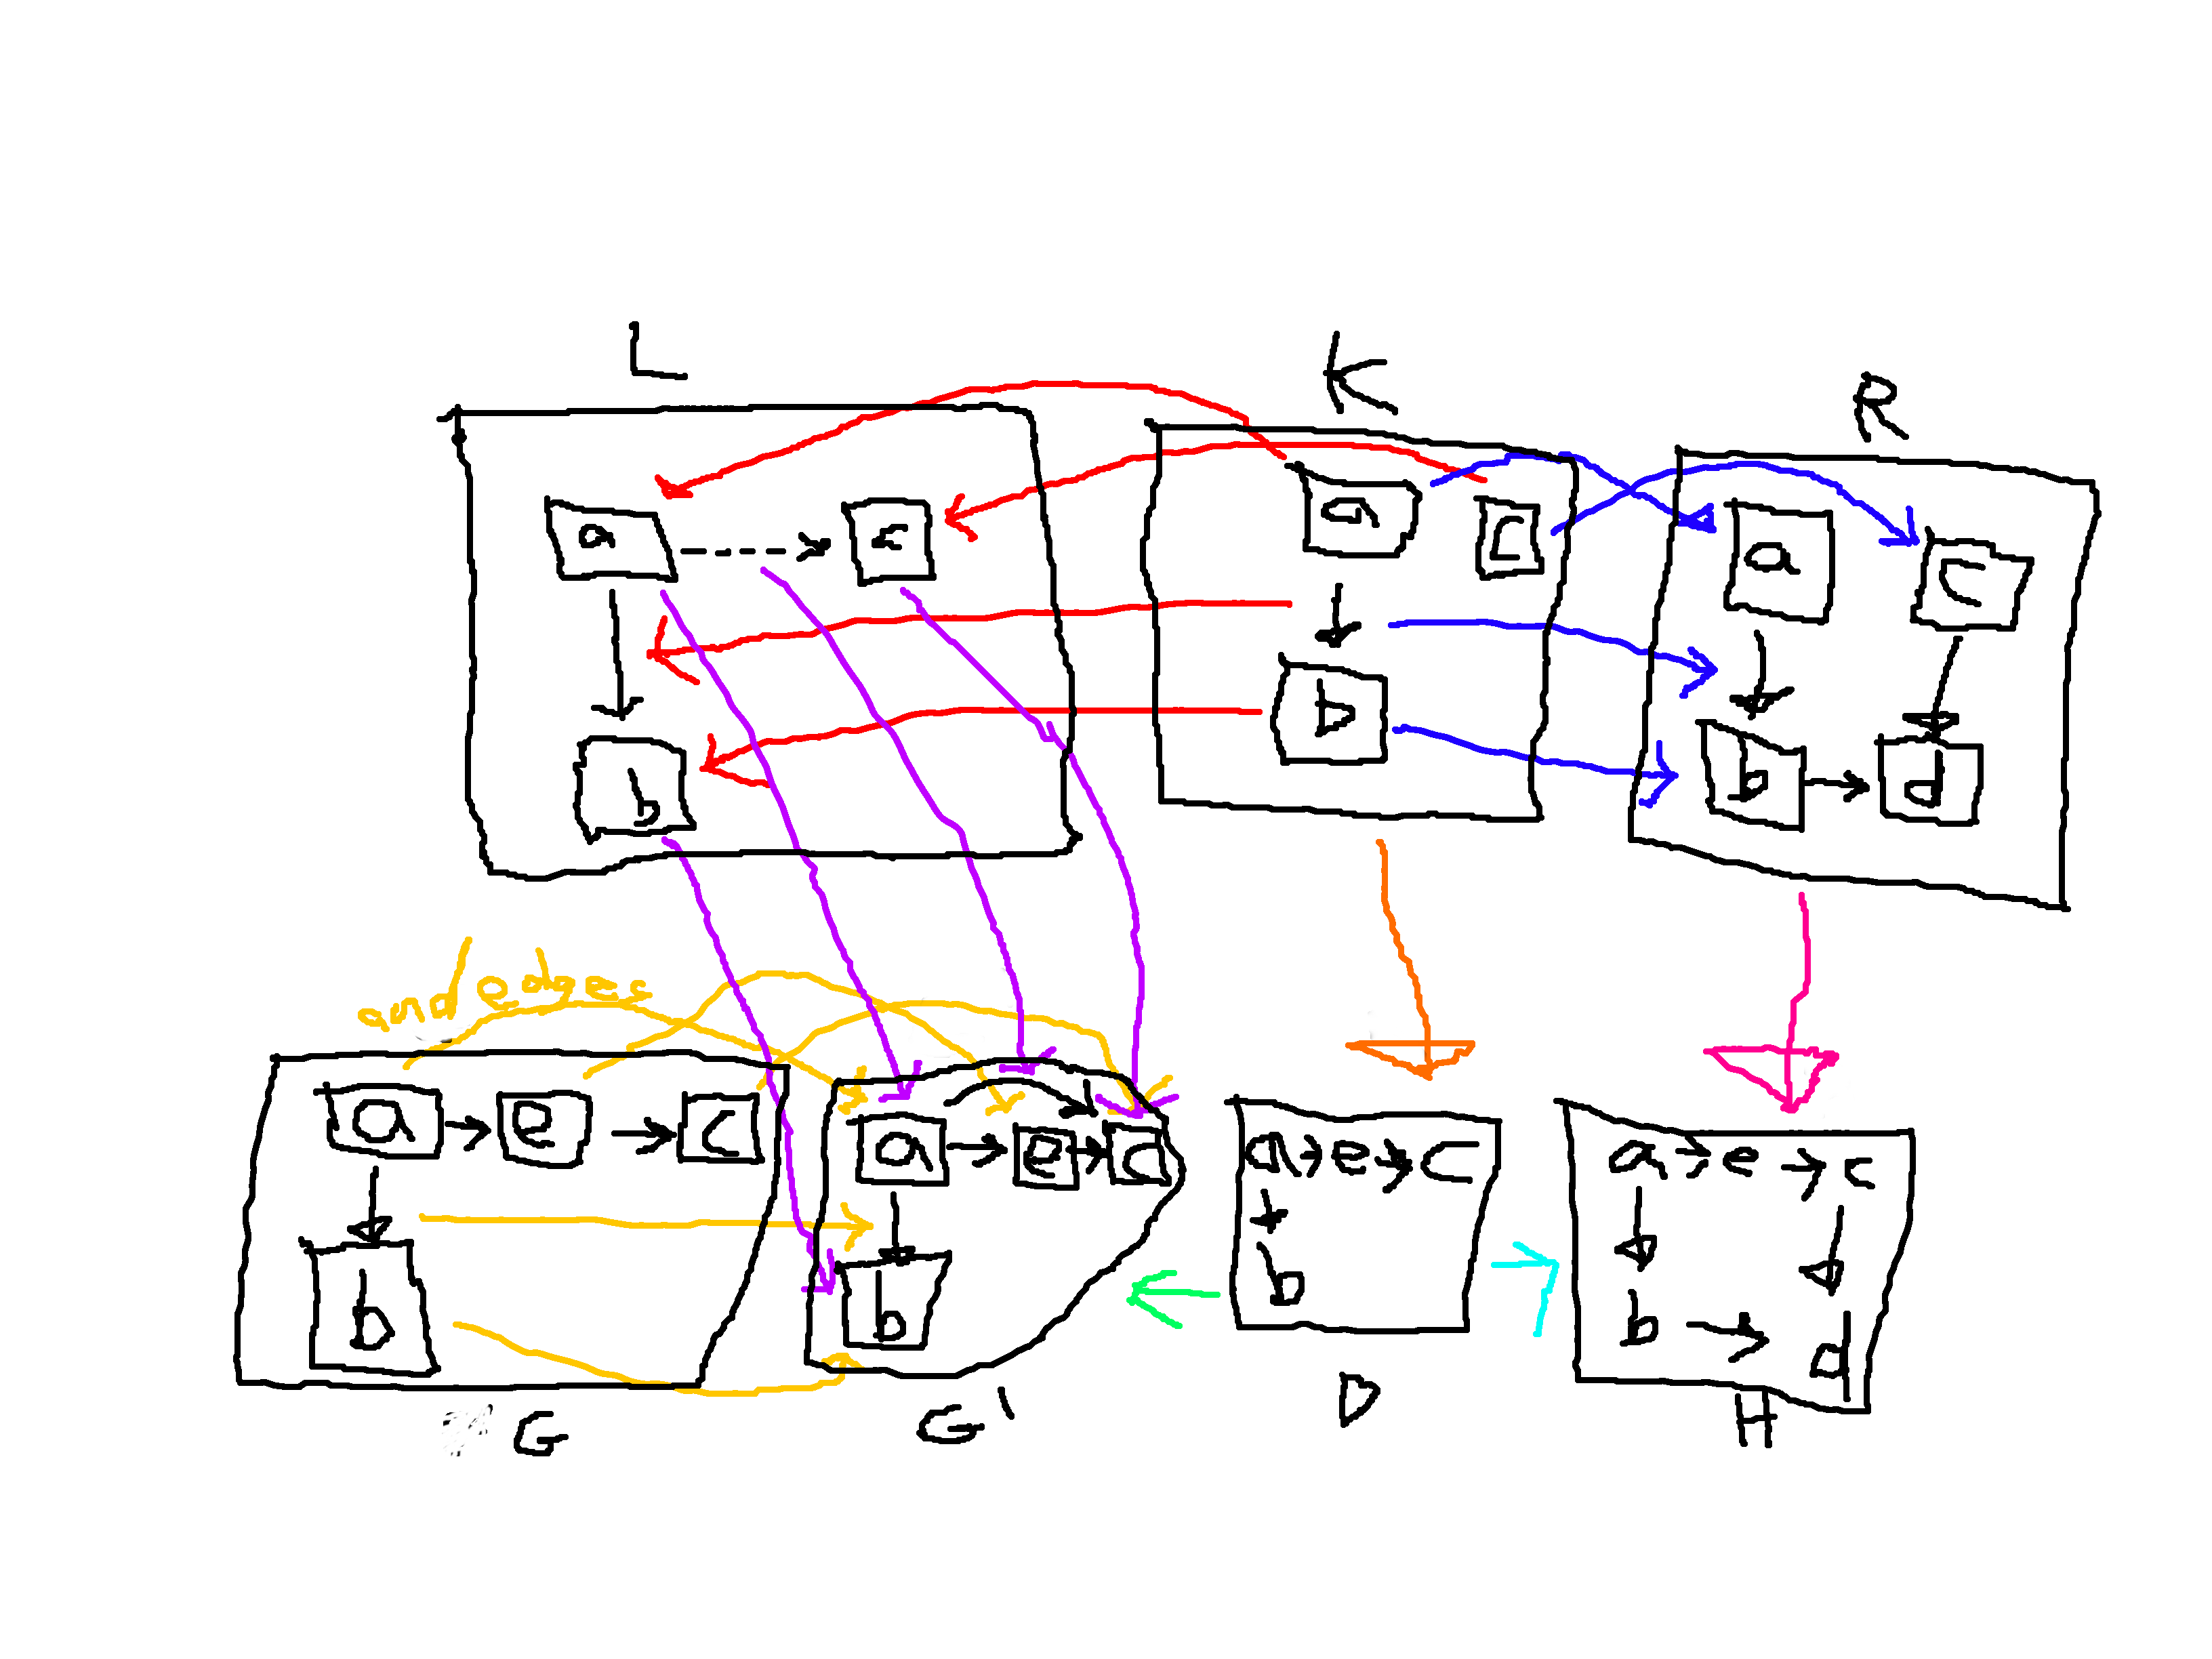
\includegraphics[width=0.44\textwidth]{figures/formal/dpo_indirect_example}
	\caption{DPO example with indirect links}
	\label{fig:dpo_indirect_example}
\end{figure}

Figure~\ref{fig:dpo_indirect_example} shows an example of the DPO approach when the rule may contain indirect links.

Note how the orange homomorphism in the bottom left does not match to the newly created edges, nor does the green homomorphism from D.

The purple homomorphism from L does match the indirect link onto the created edges. But the red homomorphism does not match onto the indirect links in L, as they do not exist in K.

\bentley{Fix this up a lot.}


\subsubsection*{DSLTrans Layer Execution}

Now that the production of a particular DSLTrans rule has been explained, the next definition defines how a DSLTrans transformation layer executes. Recall that a layer is composed of rules, and acts on the current input-output model.


\begin{definition} {DSLTrans Layer Execution}
\label{def:dsltrans_layer_execution}


The execution of a DSLTrans layer can be defined as a function as follows:

\textit{applyLayer} : IOM $\times$ Layer $\rightarrow$ IOM

Let $l = \{r_0, r_1, \dots, r_n | r_i \in \textsc{Rules}\}$, $l \in \textsc{Layers}$.

Let $\mathit{IOM}_{Input}$, $\mathit{IOM}_{Output} \in \mathit{IOMs}$.

$\mathit{IOM}_{Output}$ will be the result of applying the production \textit{p} as defined below to $\mathit{IOM}_{Input}.$

We refer to the double-pushout literature for the creation of \textit{p}. Specifically, we refer to the definition of parallel direct derivations. This p will be created out of the productions created for each of the rules $r_i$ in the layer.

$p = \big\langle (p_1, {in}^1), \dots, (p_k, {in}^k) \big\rangle : (L \xleftarrow{l} L \xrightarrow{r} R)$

This collection of the rules is possible because DSLTrans rules do not delete anything. Essentially, a union is taken of the L, K, R components of each production.
\end{definition}

\begin{figure}[h!] \centering
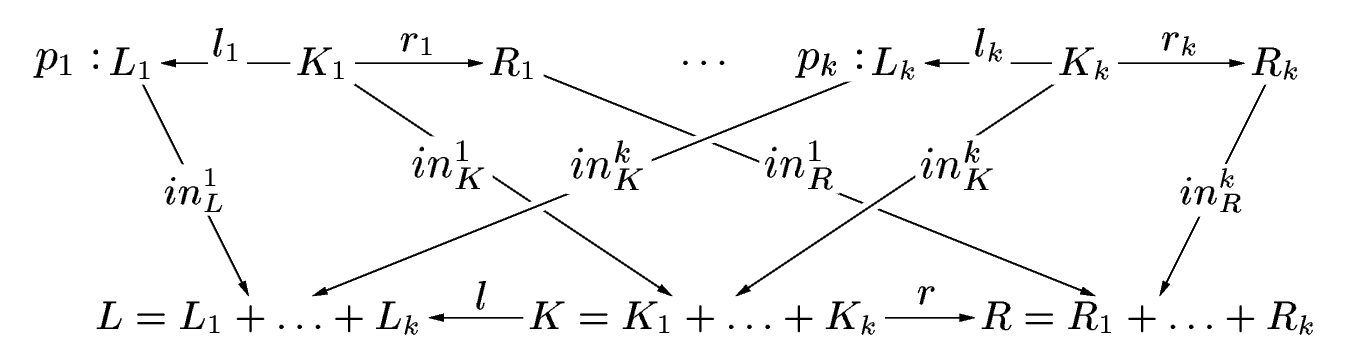
\includegraphics[width=0.44\textwidth]{figures/formal/parallel_productions}
	\caption{Parallel production \textit{p}}
	\label{fig:parallel_productions}
\end{figure}


\cref{def:dsltrans_layer_execution} is the core of DSLTrans' semantics, in which we build the result of executing a layer of a DSLTrans transformation. Many model transformation languages are based on graph rewriting, where the result of each rule rewrite is immediately usable by all other rules. In DSLTrans the result of executing one layer in DSLTrans is totally produced before the input to the layer is changed. This is enforced in \cref{def:dsltrans_layer_execution} by the fact that the layer production is composed of a union of the rule's productions. Rules belonging to the same layer are thus forced to execute independently, as described in the section on DSLTrans semantics.

\bentley{How does this handle different multiplicity of rule application?}


\subsubsection*{DSLTrans Transformation Execution}

Our final definition is for the execution of a DSLTrans transformation. Essentially, it is the chaining of layer executions applied on an input-output model.

We will begin by discussing the conditions for executing a model transformation on an input model.


\paragraph{Input Conditions}

For a well-formed transformation execution, we require the \textit{input-output model} in the domain to contain only an input graph. Recall that an \textit{input-output model} is the three-tuple $\big\langle \mathit{Input}$, $\mathit{Output}$, $\mathit{trace}\big\rangle$. We therefore require that both the $\mathit{Output}$ and $\mathit{trace}$ components in the domain IOM to be empty. This input-output model thus represents the first step of the transformation, where no rule has been executed yet.

The input-output model in the co-domain will contain this input graph, as well as the output graph and traceability links produced by the execution of the transformation. Let $\textsc{Execs}_t$ be the set of all well-formed input-output models produced for transformation $t$.

\begin{definition} {Execution of a DSLTrans Transformation\\}
\label{def:DSLTrans_transformation_execution} 

The execution of a model transformation is a function $\mathit{applyTransformation}: \mathit{IOM} \times \mathit{Transforms} \rightarrow \mathit{IOM}$.

This function is a chaining of executions of those layers within the transformation.

Recall the application of a layer is \textit{applyLayer} : IOM $\times$ Layer $\rightarrow$ IOM. Therefore, the application of a transformation is:

$\mathit{IOM}$ as input to chaining of layer executions \bentley{Is this function chaining? I don't know how to write the equation for this.}


\end{definition}


While the execution of the rules belonging to a layer happens in parallel, the execution of the layers of a transformation happens sequentially. As per \cref{def:DSLTrans_transformation_execution}, the input-output model that is the output of executing a given layer is passed onto the next layer as input. The final input-output model created will be the result of the model transformation.



\subsection{Confluence and Termination Properties}

We now prove two important properties about executions of transformations expressed in the subset of DSLTrans presented in this paper: \emph{confluence} and \emph{termination}. The proofs are provided at a high level, given the fact that DSLTrans essentially enforces both these properties by construction of the semantics of DSLTrans.

\begin{proposition}{Confluence}

Every model transformation execution is confluent up to typed graph isomorphism.

\bentley{As we are relying on the double-pushout approach, I think we get this confluence for free.}


\end{proposition}

\begin{pf}
We want to prove that for every model transformation execution of a transformation $\mathit{transform} \in \textsc{Transforms}$ having as input an input-output model $\mathit{input} \in \mathit{IOMs}$, its output is always the same up to typed graph isomorphism.\\


If we assume an execution of the transformation is not confluent then this should happen because of non-determinism when the execution of a transformation is being built. Non-determinism happens during the construction of a transformation execution at two points: 
\begin{enumerate}
\item The section `Execution of a DSLTrans Rule' discusses the matching and rewriting components to rule application. Note that our technique relies on the double-pushout approach, which itself is non-deterministic up to typed graph isomorphism, which does not contradict the proposition we are trying to prove. \bentley{Revise this.}


\item In Definition~\ref{def:dsltrans_layer_execution}, the rules composing a transformation layer are composed into a production on the input graph. Note that the order in which the transformation rules are composed may be non-deterministic. However, as these rules can be shown to be parallel independent \bentley{And they have to in that definition}, the production is by definition confluent up to typed graph isomorphism.

\end{enumerate}
Given there are no other sources of non-determinism when building the execution of a transformation, every model transformation execution is confluent up to typed graph isomorphism.
\end{pf}

\begin{proposition}{Termination}

Every model transformation execution terminates.
\end{proposition}
\begin{pf}
Let us assume that there is a transformation execution which does not terminate. In order for this to happen there must exist a part in the construction of the execution of a transformation which induces an algorithm with an infinite amount of steps. We identify three moments when this can happen:
\begin{enumerate}

\item If the matching and rewriting process of a rule is infinite. However, as the double-pushout approach uses a single production, then this must be a finite process. \bentley{Verify this, especially in the case of multiple applications of the rule.}

% if the result of the $match_{rl}(m_{in})$ function in definition~\ref{def:match_function} is an infinite set of match-apply graphs. The input-output model $m_{in}$ is by definition finite and the matching of each rule is independent from the execution of other rules in the same layer. As such, the number of subgraphs of $m_{in}$ isomorphic to $rl$'s matcher found during the execution of $rl$ is finite.


\item if Definition~\ref{def:dsltrans_layer_execution} of execution of a layer induces an infinite amount of steps. The only possibility for this to happen is if a layer has an infinite amount of transformation rules, which is a contradiction with Definition~\ref{def:layer}.

\item if Definition~\ref{def:DSLTrans_transformation_execution} of execution of a transformation induces an infinite amount of steps. Given layers are executed sequentially and no looping is allowed, the only possibility for this to happen is if the transformation has an infinite amount of layers, which contradicts Definition~\ref{def:transformation}.


\end{enumerate}
Given there are no other constructs in the semantics of a transformation that can induce an infinite amount of steps, every model transformation execution terminates.
\end{pf}